\section{Cryptanalysis}
\begin{frame}{Differential \& Linear Attack}
    \begin{itemize}
         \item  Finding total number of active S-Box 
         \pause
         \item Construct a mixed integer linear programming (MILP).
         \pause
         \item All variables corresponding to the inputs of the
                SubCells operations are summed in the objective function,
                    so this corresponds to the number of active S-boxes\footnote{N. Mouha, Q. Wang, D. Gu, and B. Preneel, ‘‘Differential and linear
cryptanalysis using mixed-integer linear programming,’’ in Proc. 7th Int.
Conf. Inf. Secur. Cryptol., vol. 7537, 2011, pp. 57–76.}
    \end{itemize}
\end{frame}

\begin{frame}{Differential \& Linear Attack}
\begin{center}
    \scalebox{0.9}{$\begin{bmatrix} x_0 & x_4 & x_8 & x_{12}\\ x_1 & x_5 & x_9 & x_{13}\\
     x_2 & x_6 & x_{10} & x_{14}\\ x_3 & x_7 & x_{11} & x_{15} \end{bmatrix}$
    $\xrightarrow{\text{SC}}$
    $\begin{bmatrix} x_0 & x_4 & x_8 & x_{12}\\ x_1 & x_5 & x_9 & x_{13}\\
    x_2 & x_6 & x_{10} & x_{14}\\ x_3 & x_7 & x_{11} & x_{15} \end{bmatrix}$
    $\xrightarrow{\text{Mix Row}}$
    $\begin{bmatrix} x_{16} & x_{17} & x_{18} & x_{19}\\ x_{20} & x_{21} & x_{22} & x_{23}\\
    x_{24} & x_{25} & x_{26} & x_{27}\\ x_{28} & x_{29} & x_{30} & x_{31} \end{bmatrix}$} \\
    
    \vspace{1cm}
    \scalebox{0.9}{
    $\xrightarrow{\text{Mix column}}$
    $\begin{bmatrix} x_{32} & x_{36} & x_{40} & x_{44}\\ x_{33} & x_{37} & x_{41} & x_{45}\\
    x_{34} & x_{38} & x_{42} & x_{46}\\ x_{35} & x_{39} & x_{43} & x_{47} \end{bmatrix}$
    $\xrightarrow{\text{SC}}$
    $\begin{bmatrix} x_{32} & x_{36} & x_{40} & x_{44}\\ x_{33} & x_{37} & x_{41} & x_{45}\\
    x_{34} & x_{38} & x_{42} & x_{46}\\ x_{35} & x_{39} & x_{43} & x_{47} \end{bmatrix}$}
    
\end{center}
\end{frame}


\begin{frame}{Differential \& Linear Attack}
    \begin{itemize}
         \item  The MixRows can be constrained by the following linear equations:
    \end{itemize}
    \begin{gather}
        x_0+x_1+x_2+x_3+x_{16}+x_{20}+x_{24}+x_{28}-5d_0 \ge0\\
        x_4+x_5+x_6+x_7+x_{17}+x_{21}+x_{25}+x_{29}-5d_1\ge0\\
        x_8+x_9+x_{10}+x_{11}+x_{18}+x_{22}+x_{26}+x_{30}-5d_2\ge0\\
        x_{12}+x_{13}+x_{14}+x_{15}+x_{19}+x_{23}+x_{27}+x_{31}-5d_3\ge0
    \end{gather}
\end{frame}

\begin{frame}{Differential \& Linear Attack}
    \begin{itemize}
         \item  The MixColumns can be constrained by the following linear equations: 
    \end{itemize}
    \begin{gather}
        x_{16}+x_{17}+x_{18}+x_{19}+x_{32}+x_{33}+x_{34}+x_{35}-5d_4\ge0\\
        x_{20}+x_{21}+x_{22}+x_{23}+x_{36}+x_{37}+x_{38}+x_{39}-5d_5\ge0\\
        x_{24}+x_{25}+x_{26}+x_{27}+x_{40}+x_{41}+x_{42}+x_{43}-5d_6\ge0\\
        x_{28}+x_{29}+x_{30}+x_{31}+x_{44}+x_{45}+x_{46}+x_{47}-5d_7\ge0
    \end{gather}

\end{frame}

\begin{frame}{Differential \& Linear Attack}
    \begin{figure}[htp]
        \centering
        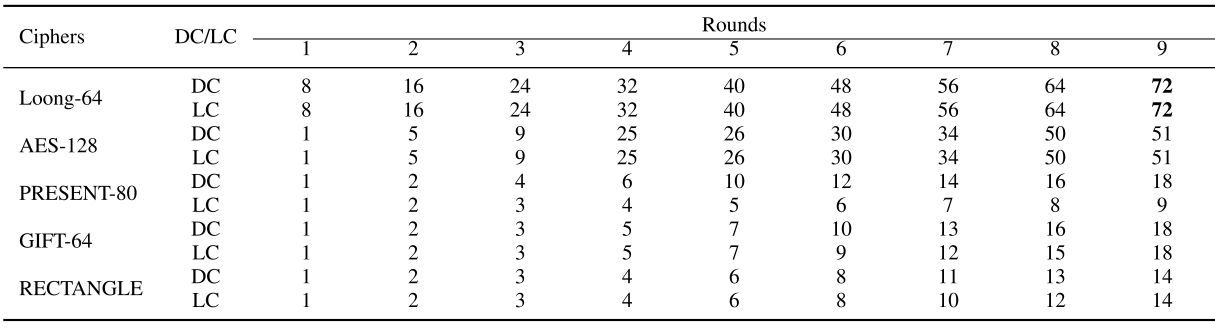
\includegraphics[width=10cm]{a1f.png}
        \caption{The number of active S-boxes.}
    \end{figure}
    \begin{itemize}
    \pause
         \item Loong has more active S-Box Compare to other Block ciphers.
    \end{itemize}
\end{frame}

\begin{frame}{Differential \& Linear Attack}
    \begin{itemize}
         \item Loong-64 has 16 rounds, and its differential probability is $2^{-256}$
and its bias of linear probability is $2^{-129}$ .\\
\pause
        \item Loong-80 has 20 rounds, and its differential probability is $2^{-320}$ and its bias
of linear probability is $2^{-161}$ .\\
\pause
        \item And Loong-128 has 32 rounds, and its differential probability is $2^{-512}$ and its bias of linear probability is $2^{-257}$
    \end{itemize}
    Therefore, Loong has high security and
we believe Loong is enough to resist against differential and
linear attacks.
\end{frame}



\begin{frame}{Related-key Attack}
    \begin{itemize}
        \item Analyze the probability of related-key differential characteristics.
        \pause
        \item Differences are inserted in the round key input the round key will be active in Loong-64.
    \end{itemize}
    \begin{center}
      $\TeaserImage{a1b.png} \xrightarrow{\text{SC}} \TeaserImage{a1b.png}
        \xrightarrow{\text{MixRow}} \TeaserImage{3.png} $
        $\xrightarrow{\text{MixColumn}}
        \TeaserImage{a1d.png} \xrightarrow{\text{SC}}\TeaserImage{a1d.png}$
    \end{center}
\end{frame}

\begin{frame}{Related-key Attack}
    \begin{itemize}
        \item Loong-64 has at least (RN /2) × 8 active S-boxes in related-key differential path.
        \pause
        \item And Loong 8-round differential probability is $2^{-64}$

    \end{itemize}
\end{frame}


\begin{frame}{Algebraic Attack}
    \begin{itemize}
        \item Used to find multi-variable equation for non-linear component
        \pause
        \item Loong uses sub-cell two times in one round 
        \pause
        \item Each sub-cell uses 16(block size) s-boxes
        \pause
        \item Loong uses 32(16*2) sboxes in each round
        \pause
        \item Loong-64 uses 512 sboxes 
        \pause
        \item Loong-80 uses 640 sboxes
        \pause
        \item Loong-128 uses 1024 sboxes
    \end{itemize}
\end{frame}

\begin{frame}{Algebraic Attack}
    \begin{itemize}
        \item A 4 × 4 S-box can be described by 21 quadratic equations of 8 input/output-bit variables over\footnote{N. T. Courtois and J. Pieprzyk, ‘‘Cryptanalysis of block ciphers with
overdefined systems of equations,’’ in Proc. 8th Int. Conf. Theory Appl.
Cryptol. Inf. Secur., vol. 2501, 2002, pp. 267–287}
    \end{itemize}
\end{frame}

\begin{frame}{Algebraic Attack}
    \begin{itemize}
        \item Using that fact here is the comparison of Loong with other Lightweight ciphers\\ \vspace{0.6cm}
    \scalebox{0.8}{
    \begin{table}[]
        \centering
        \begin{tabular}{ |c|c|c|c|c|  } \hline \multicolumn{5}{|c|}{The Algebraic Comparison information in different ciphers} \\ \hline Ciphers &Rounds &S-boxes &Quadratic equations &Variables\\ \hline Loong-64 &16 &512 &10752    &4096\\ Loong-80 &20 &\textbf{640} &\textbf{13440} &\textbf{5120}\\ Loong-128 &32 &\textbf{1024} &\textbf{21504} &\textbf{8192}\\ KLEIN-64 &12 &240 &5040 &1920\\ MIBS-80 &32 &320 &6720 &2560\\ PRESENT-80 &31 &527 &11067 &4216\\ \hline 
        \end{tabular}
    \end{table}
        
        }
    \end{itemize}
\end{frame}

\begin{frame}{Meet-in-The-Middle Attack}
    \begin{itemize}
        \item Known Plain-text Attack (KPA)
        \pause
        \item Analytical method to balancing time and memory
        \pause
        \item Loong round function has faster diffusion effect
        \pause
        \item Fully diffused in two round of encryption
        \pause
        \item In the worst case, meet in the middle attack can analyze up to 7(2+2+3=7) rounds.
    \end{itemize}
    \vspace{1cm}
    \textbf{Secure against MITM Attack}
\end{frame}